\documentclass{article}
% Change "article" to "report" to get rid of page number on title page
\usepackage{amsmath,amsfonts,amsthm,amssymb}
\usepackage{setspace}
\usepackage{Tabbing}
\usepackage{fancyhdr}
\usepackage{lastpage}
\usepackage{extramarks}
\usepackage{chngpage}
\usepackage{soul,color}
\usepackage{graphicx,float,wrapfig}
\usepackage{listings}

% In case you need to adjust margins:
\topmargin=-0.45in      %
\evensidemargin=0in     %
\oddsidemargin=0in      %
\textwidth=6.5in        %
\textheight=9.0in       %
\headsep=0.25in         %

% Homework Specific Information
\newcommand{\hmwkTitle}{Homework 2}
\newcommand{\hmwkDueDate}{Feb 14, 2013}
\newcommand{\hmwkClass}{Bayesian Statistical Methods}
\newcommand{\hmwkClassTime}{}
\newcommand{\hmwkClassInstructor}{}
\newcommand{\hmwkAuthorName}{Andrew Kurzawski}

% Setup the header and footer
\pagestyle{fancy}                                                       %
\lhead{\hmwkAuthorName}                                                 %
\chead{\hmwkClass\ (\hmwkClassInstructor\ \hmwkClassTime): \hmwkTitle}  %
\rhead{\firstxmark}                                                     %
\lfoot{\lastxmark}                                                      %
\cfoot{}                                                                %
\rfoot{Page\ \thepage\ of\ \pageref{LastPage}}                          %
\renewcommand\headrulewidth{0.4pt}                                      %
\renewcommand\footrulewidth{0.4pt}                                      %

% This is used to trace down (pin point) problems
% in latexing a document:
%\tracingall

%%%%%%%%%%%%%%%%%%%%%%%%%%%%%%%%%%%%%%%%%%%%%%%%%%%%%%%%%%%%%
% Some tools
\newcommand{\enterProblemHeader}[1]{\nobreak\extramarks{#1}{#1 continued on next page\ldots}\nobreak%
                                    \nobreak\extramarks{#1 (continued)}{#1 continued on next page\ldots}\nobreak}%
\newcommand{\exitProblemHeader}[1]{\nobreak\extramarks{#1 (continued)}{#1 continued on next page\ldots}\nobreak%
                                   \nobreak\extramarks{#1}{}\nobreak}%

\newlength{\labelLength}
\newcommand{\labelAnswer}[2]
  {\settowidth{\labelLength}{#1}%
   \addtolength{\labelLength}{0.25in}%
   \changetext{}{-\labelLength}{}{}{}%
   \noindent\fbox{\begin{minipage}[c]{\columnwidth}#2\end{minipage}}%
   \marginpar{\fbox{#1}}%

   % We put the blank space above in order to make sure this
   % \marginpar gets correctly placed.
   \changetext{}{+\labelLength}{}{}{}}%

\setcounter{secnumdepth}{0}
\newcommand{\homeworkProblemName}{}%
\newcounter{homeworkProblemCounter}%
\newenvironment{homeworkProblem}[1][Problem \arabic{homeworkProblemCounter}]%
  {\stepcounter{homeworkProblemCounter}%
   \renewcommand{\homeworkProblemName}{#1}%
   \section{\homeworkProblemName}%
   \enterProblemHeader{\homeworkProblemName}}%
  {\exitProblemHeader{\homeworkProblemName}}%

\newcommand{\problemAnswer}[1]
  {\noindent\fbox{\begin{minipage}[c]{\columnwidth}#1\end{minipage}}}%

\newcommand{\problemLAnswer}[1]
  {\labelAnswer{\homeworkProblemName}{#1}}

\newcommand{\homeworkSectionName}{}%
\newlength{\homeworkSectionLabelLength}{}%
\newenvironment{homeworkSection}[1]%
  {% We put this space here to make sure we're not connected to the above.
   % Otherwise the changetext can do funny things to the other margin

   \renewcommand{\homeworkSectionName}{#1}%
   \settowidth{\homeworkSectionLabelLength}{\homeworkSectionName}%
   \addtolength{\homeworkSectionLabelLength}{0.25in}%
   \changetext{}{-\homeworkSectionLabelLength}{}{}{}%
   \subsection{\homeworkSectionName}%
   \enterProblemHeader{\homeworkProblemName\ [\homeworkSectionName]}}%
  {\enterProblemHeader{\homeworkProblemName}%

   % We put the blank space above in order to make sure this margin
   % change doesn't happen too soon (otherwise \sectionAnswer's can
   % get ugly about their \marginpar placement.
   \changetext{}{+\homeworkSectionLabelLength}{}{}{}}%

\newcommand{\sectionAnswer}[1]
  {% We put this space here to make sure we're disconnected from the previous
   % passage

   \noindent\fbox{\begin{minipage}[c]{\columnwidth}#1\end{minipage}}%
   \enterProblemHeader{\homeworkProblemName}\exitProblemHeader{\homeworkProblemName}%
   \marginpar{\fbox{\homeworkSectionName}}%

   % We put the blank space above in order to make sure this
   % \marginpar gets correctly placed.
   }%

% Python Setup
\lstset{
  language=Python,
  showstringspaces=false,
  formfeed=\newpage,
  tabsize=4,
  commentstyle=\itshape,
  basicstyle=\ttfamily,
  morekeywords={models, lambda, forms}
}

% Uncomment lines and make changes to have a header
\newcommand{\code}[1]{ % change to [2]
  % \hrulefill
  % \subsection*{#1}
  \lstinputlisting{#1} % change to {#2}
  \vspace{2em}
}

%%%%%%%%%%%%%%%%%%%%%%%%%%%%%%%%%%%%%%%%%%%%%%%%%%%%%%%%%%%%%


%%%%%%%%%%%%%%%%%%%%%%%%%%%%%%%%%%%%%%%%%%%%%%%%%%%%%%%%%%%%%
% Make title
\title{\vspace{2in}\textmd{\textbf{\hmwkClass:\ \hmwkTitle}}\\\normalsize\vspace{0.1in}\small{Due\ on\ \hmwkDueDate}\\\vspace{0.1in}\large{\textit{\hmwkClassInstructor\ \hmwkClassTime}}\vspace{3in}}
\date{}
\author{\textbf{\hmwkAuthorName}}
%%%%%%%%%%%%%%%%%%%%%%%%%%%%%%%%%%%%%%%%%%%%%%%%%%%%%%%%%%%%%

\begin{document}
\begin{spacing}{1.1}
\maketitle
\newpage
% Uncomment the \tableofcontents and \newpage lines to get a Contents page
% Uncomment the \setcounter line as well if you do NOT want subsections
%       listed in Contents
%\setcounter{tocdepth}{1}
%\tableofcontents
%\newpage

% When problems are long, it may be desirable to put a \newpage or a
% \clearpage before each homeworkProblem environment

\clearpage
\begin{homeworkProblem}
Reading Assignment.
\end{homeworkProblem}


\begin{homeworkProblem}

I began by doing a test run of 1000 iterations with no burn in or thinning. From the traces of $\mu$ and $\sigma$, I saw that both had converged within a few iterations. So, I burned 100 iterations because running the model is not computationally expensive. Then, I ran the model again and observed significant autocorrelation of $\mu$ within about 15 itterations, so I selected to thin the results by 15. Fig.~\ref{fig:p2_mu} and Fig.~\ref{fig:p2_sigma} are the resulting posterior summaries after 10,000 iterations.

\begin{figure}[ht]
\begin{center}
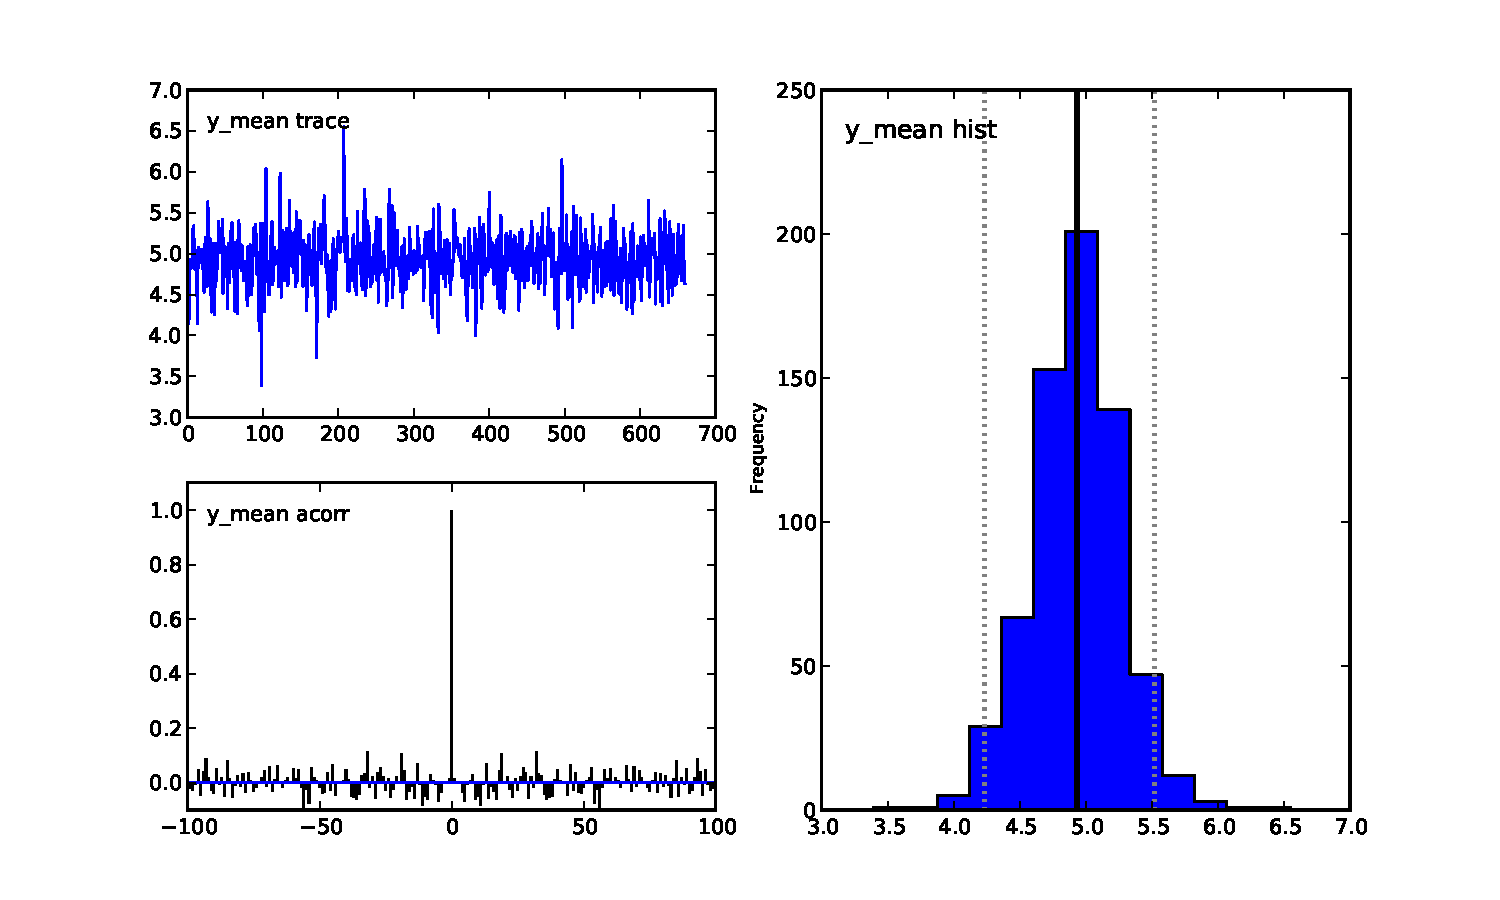
\includegraphics[height=2.75in]{./Figures/Prob2/y_mean}
\end{center}
\caption{Posterior summary for $\mu$ using PyMC}
\label{fig:p2_mu}
\end{figure}

\begin{figure}[ht]
\begin{center}
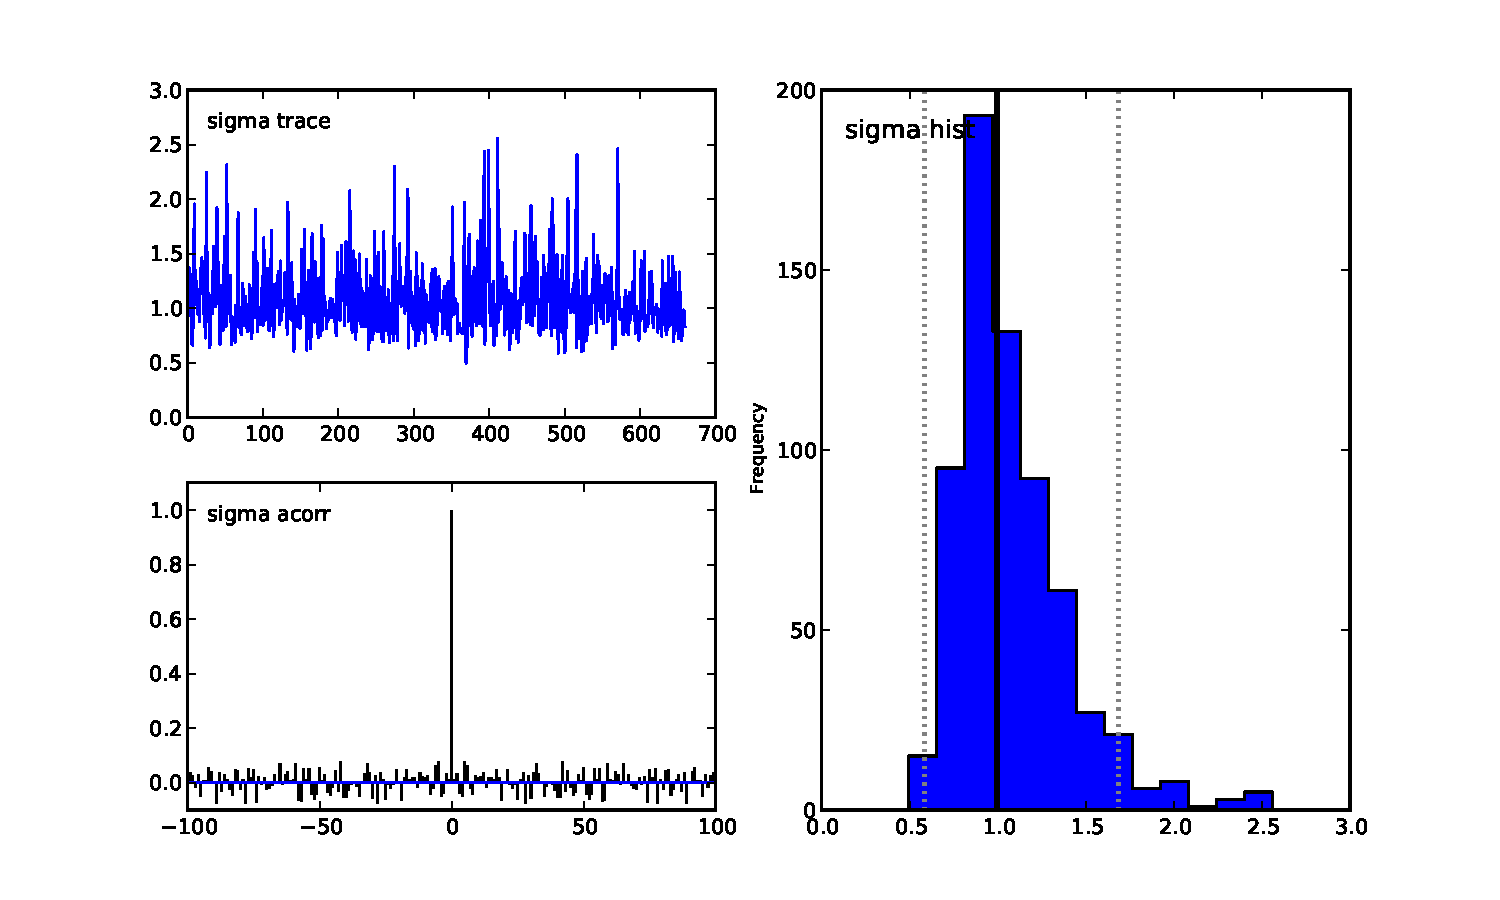
\includegraphics[height=2.75in]{./Figures/Prob2/sigma}
\end{center}
\caption{Posterior summary for $\sigma$ using PyMC}
\label{fig:p2_sigma}
\end{figure}

\end{homeworkProblem}


\begin{homeworkProblem}

In a standard slice sampler, you would pick a starting value for $\theta$. However, because in this case we are able to sample off of $h_1(\theta)$, we can choose the starting value for our chain by sampling from this distribution. This in turn cuts down on the burn in time. From here, we would proceed with slice sampling as follows:

Use $\theta_0$ generated from $h_1(\theta)$ to calculate $h(\theta_0) = h_1(\theta_0) h_2(\theta_0)$.

Sample $U$ from $Uniform (0, h(\theta_0))$.

Search for the intercepts of $U$ and $h(\theta_0)$, denoted as $\theta_L$ and $\theta_R$.

Sample $\theta_1$ from $Uniform (\theta_L, \theta_R)$.

Repeat.

\end{homeworkProblem}


\begin{homeworkProblem}

The following code is a Metropolis-Hastings algorithm written in Python for the data given in Problem 2 with $\sigma = 1$. A poster summary for $\mu$ is given in Fig.~\ref{fig:p4_mu} for 10000 iterations. Roughly 10\% of the samples were accepted.

\code{./Scripts/mh_sampler.py}

\begin{figure}[ht]
\begin{center}
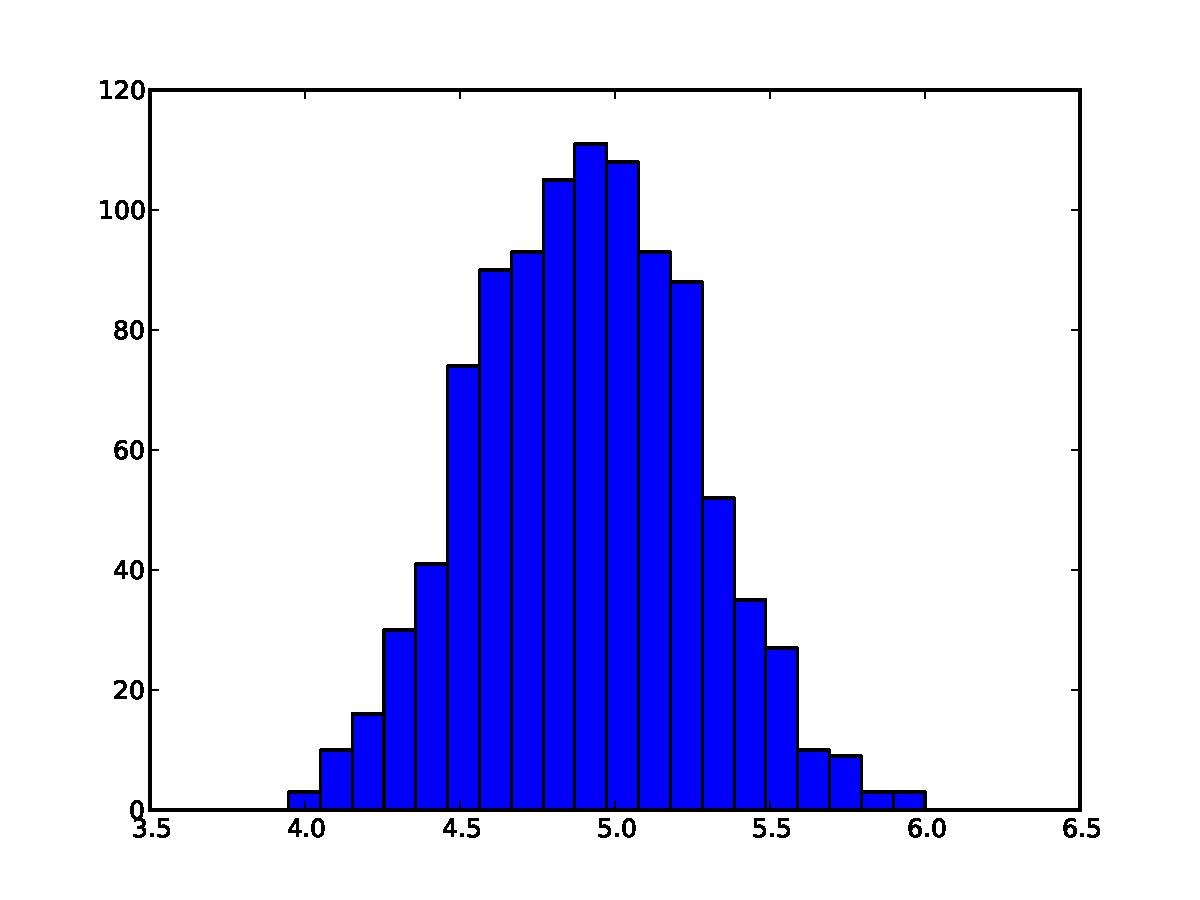
\includegraphics[height=3.0in]{./Figures/Prob4/mu_hist}
\end{center}
\caption{Posterior summary for $\mu$ using Metropoils-Hastings}
\label{fig:p4_mu}
\end{figure}

\end{homeworkProblem}


\begin{homeworkProblem}

The following code is a Slice Sampling algorithm written in Python for the data given in Problem 2 with $\sigma = 1$. A poster summary for $\mu$ is given in Fig.~\ref{fig:p5_mu} for 10000 iterations.

\code{./Scripts/slice_sampler.py}

\begin{figure}[ht]
\begin{center}
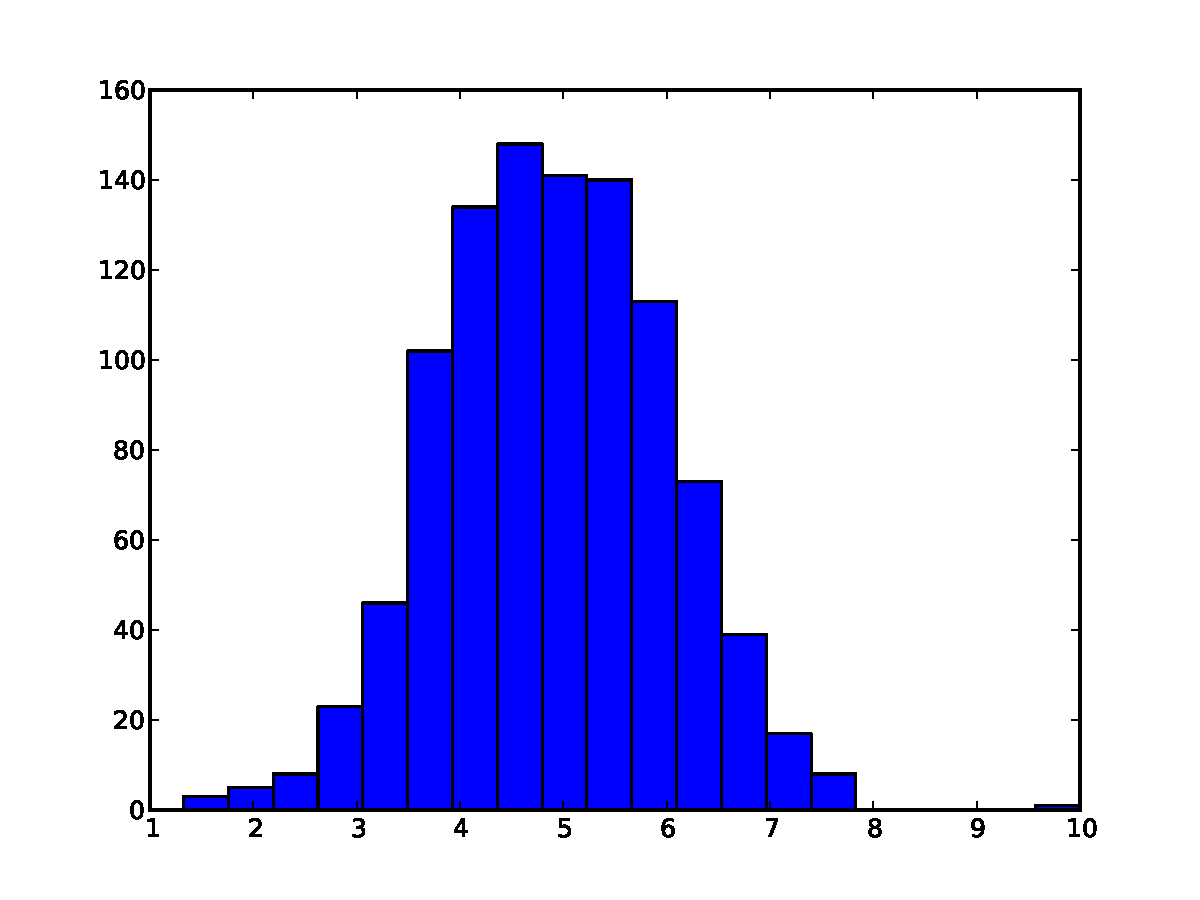
\includegraphics[height=3.0in]{./Figures/Prob5/mu_hist}
\end{center}
\caption{Posterior summary for $\mu$ using Slice Sampling}
\label{fig:p5_mu}
\end{figure}

\end{homeworkProblem}


\begin{homeworkProblem}

I used the same methods stated in Problem 2 to choose the Burn In and Thinning for each case. The main differences to take note of between the posteriors (Fig.~\ref{fig:p6_a}-\ref{fig:p6_c}) are that the means sampled from the Informed and Uniform priors are both slightly higher than that of the diffuse Gamma prior. Additionally, the posterior generated from the Uniform prior has a larger tail on the right hand side, due to the fact that the Uniform prior was given the range from 0 to 20.

\begin{table}[h]
\caption{Comparison of Specified Priors}
\begin{center}
  \begin{tabular}{cccc}
    \hline\noalign{\smallskip}
    Prior & Iterations & Burn In & Thinning \\
    \noalign{\smallskip}\hline\noalign{\smallskip}
    Diffuse Gamma(0.001,0.001) & 50,000 & 10,000 & 20\\
    Informed Gamma(1.11,1.61) & 30,000 & 10,000 & 20\\ 
    Uniform(0,20) & 30,000 & 4,000 & 15\\ 
    \noalign{\smallskip}\hline
  \end{tabular}
\end{center}
\label{tab_p6}
\end{table}

The effect of assigning a Uniform prior becomes much more apparent when we examine the probability that $\theta$ is greater than 0.5 (Tab.~\ref{tab_p6_b}).

\begin{table}[h]
\caption{Probablity that $\theta$ is greater than 0.5}
\begin{center}
  \begin{tabular}{cccc}
    \hline\noalign{\smallskip}
    Prior & Probability \\
    \noalign{\smallskip}\hline\noalign{\smallskip}
    Diffuse Gamma(0.001,0.001) & 0.0065\\
    Informed Gamma(1.11,1.61) & 0.006\\ 
    Uniform(0,20) & 0.0179\\ 
    \noalign{\smallskip}\hline
  \end{tabular}
\end{center}
\label{tab_p6_b}
\end{table}

\begin{figure}[h!]
\begin{center}
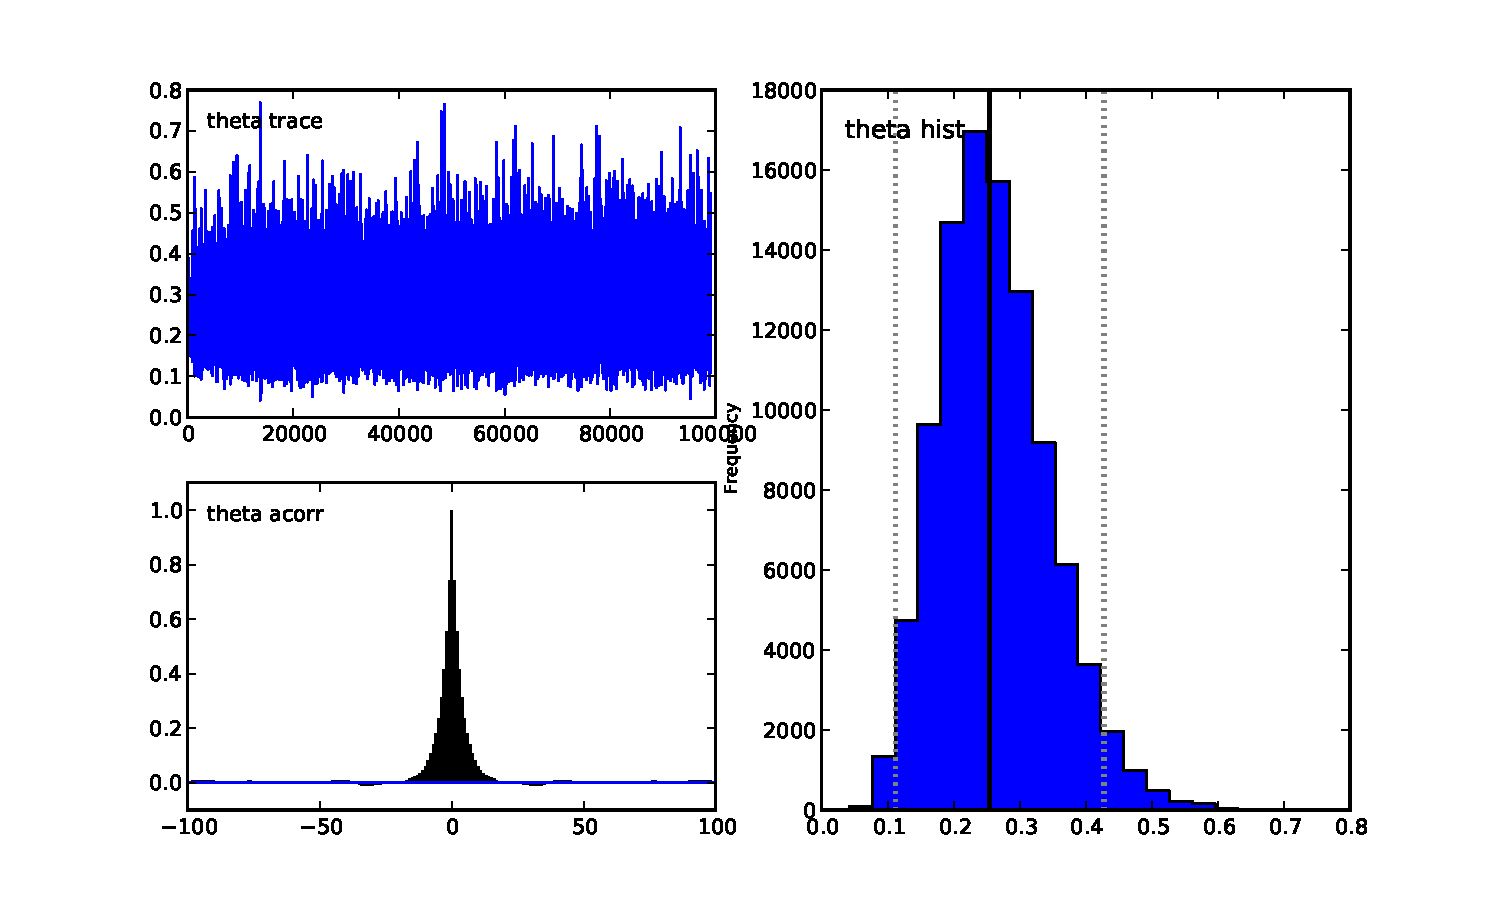
\includegraphics[height=3.0in]{./Figures/Prob6/A/theta}
\end{center}
\caption{Posterior summary for $\theta$ using a diffuse gamma prior}
\label{fig:p6_a}
\end{figure}

\begin{figure}[h!]
\begin{center}
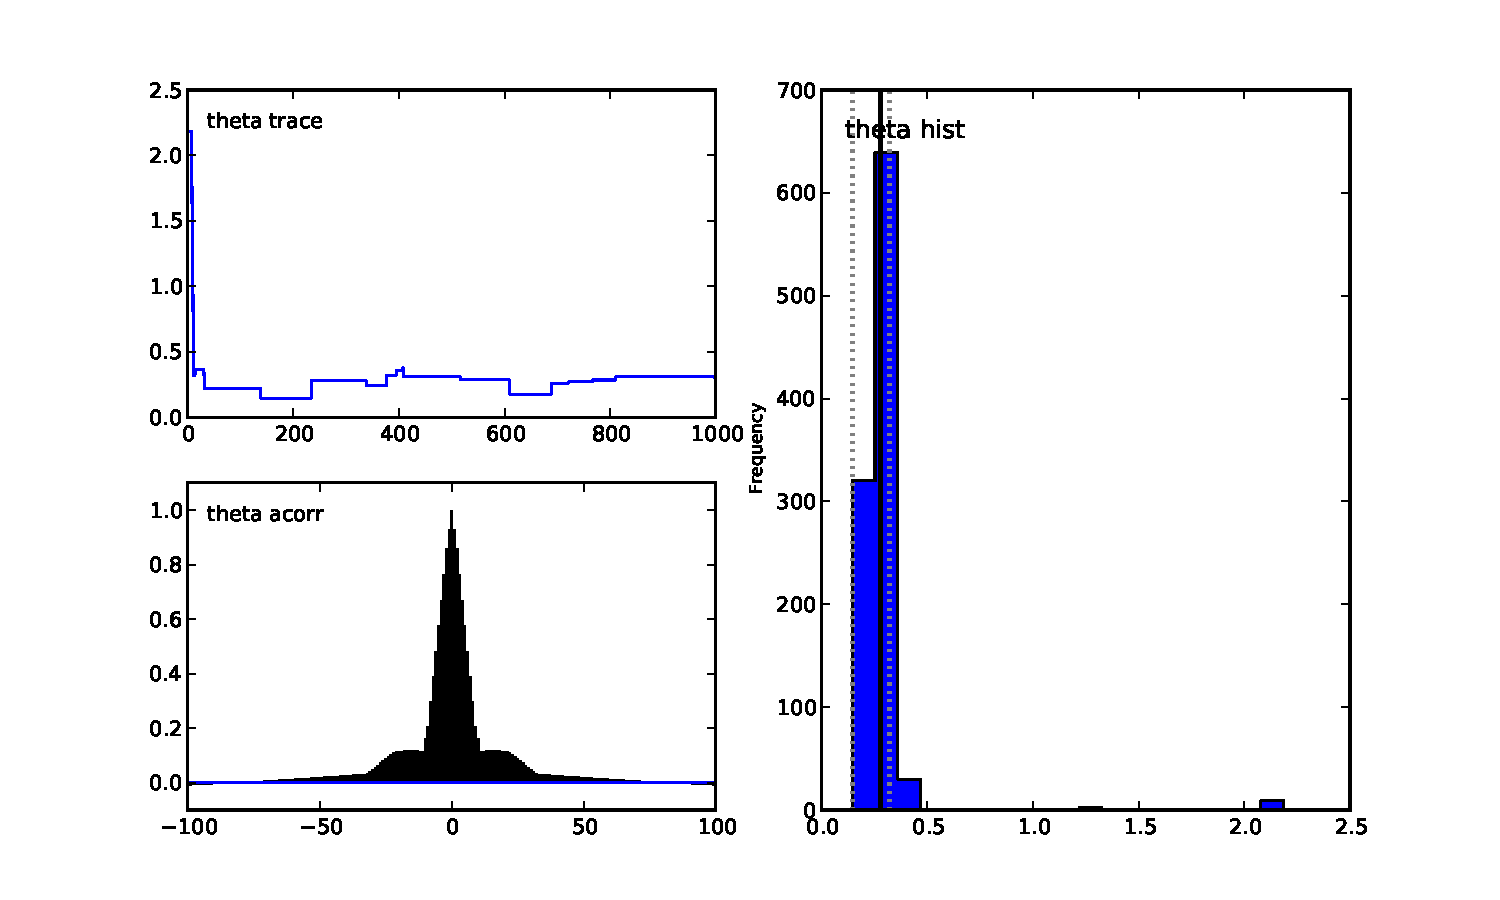
\includegraphics[height=3.0in]{./Figures/Prob6/B/theta}
\end{center}
\caption{Posterior summary for $\theta$ using an informed gamma prior}
\label{fig:p6_b}
\end{figure}

\begin{figure}[h!]
\begin{center}
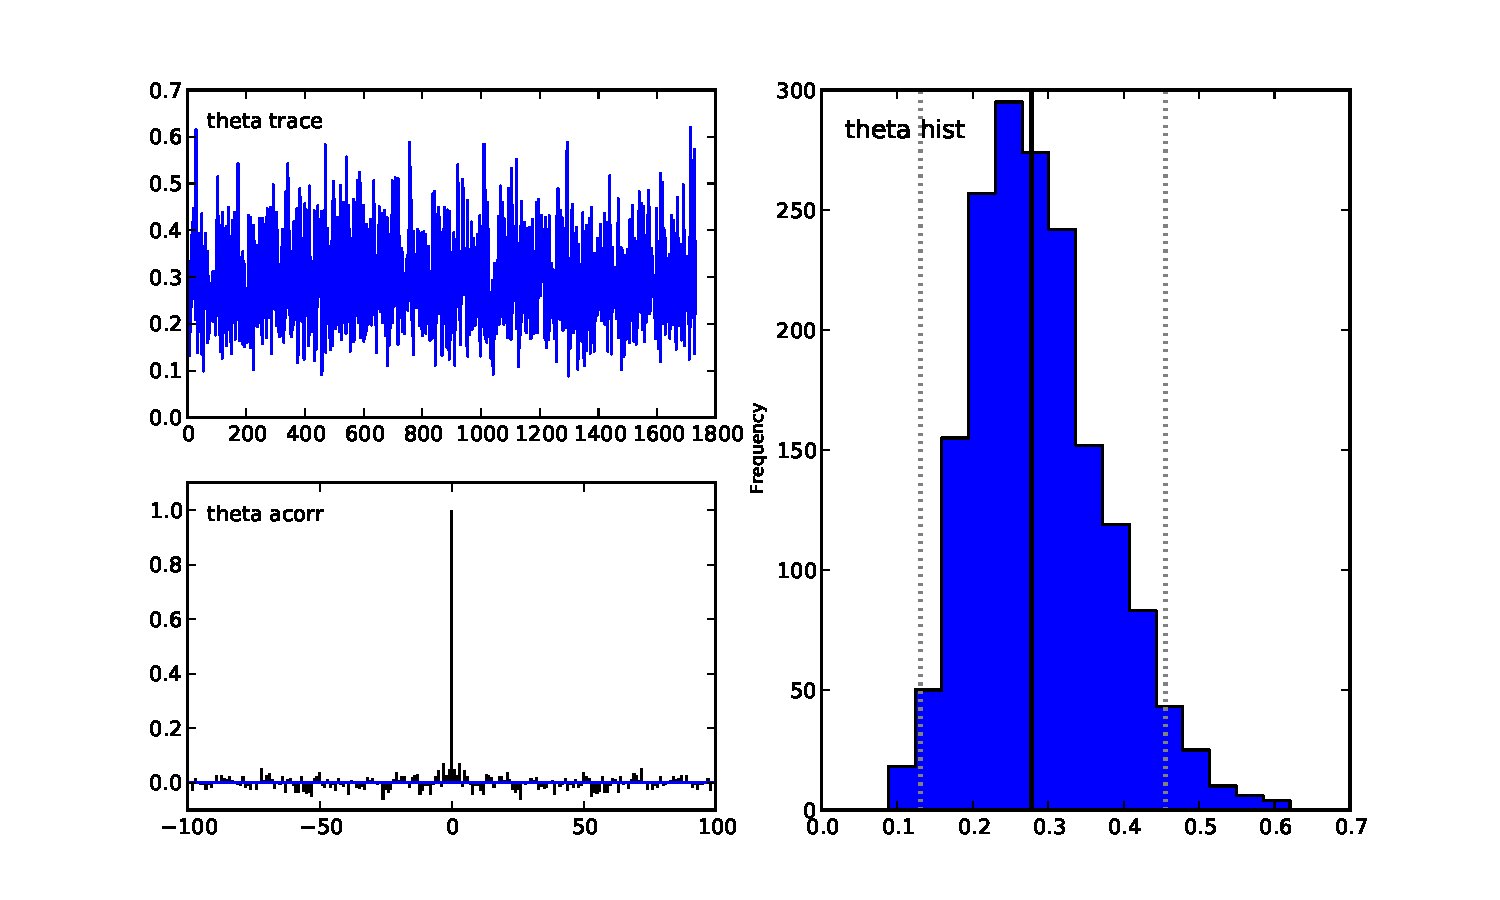
\includegraphics[height=3.0in]{./Figures/Prob6/C/theta}
\end{center}
\caption{Posterior summary for $\theta$ using a uniform prior}
\label{fig:p6_c}
\end{figure}

\end{homeworkProblem}


\begin{homeworkProblem}

Once again, Burn In and Thinning were determined in the same fashion as Problem 2, with the main difference being that I had to examine multiple posterior distributions for convergence and autocorrelation. Upon looking at the means of $\mu$, I realized that the multivariate normal distribution was not working properly. I am probably specifying something incorrectly. Including any further analysis at this point would be useless, however I will run the model again in my free time once I figure out how to properly implement a multivariate normal distribution in PyMC.

\begin{table}[h]
\caption{Burn In and Thinning for Informed and Uninformed Priors}
\begin{center}
  \begin{tabular}{cccc}
    \hline\noalign{\smallskip}
    Priors & Burn In & Thinning \\
    \noalign{\smallskip}\hline\noalign{\smallskip}
    Informed & 20,000 & 15\\
    Uninformed & 10,000 & 25\\ 
    \noalign{\smallskip}\hline
  \end{tabular}
\end{center}
\label{tab_p7}
\end{table}

\begin{table}[h!]
\begin{center}
\begin{tabular}{cc}
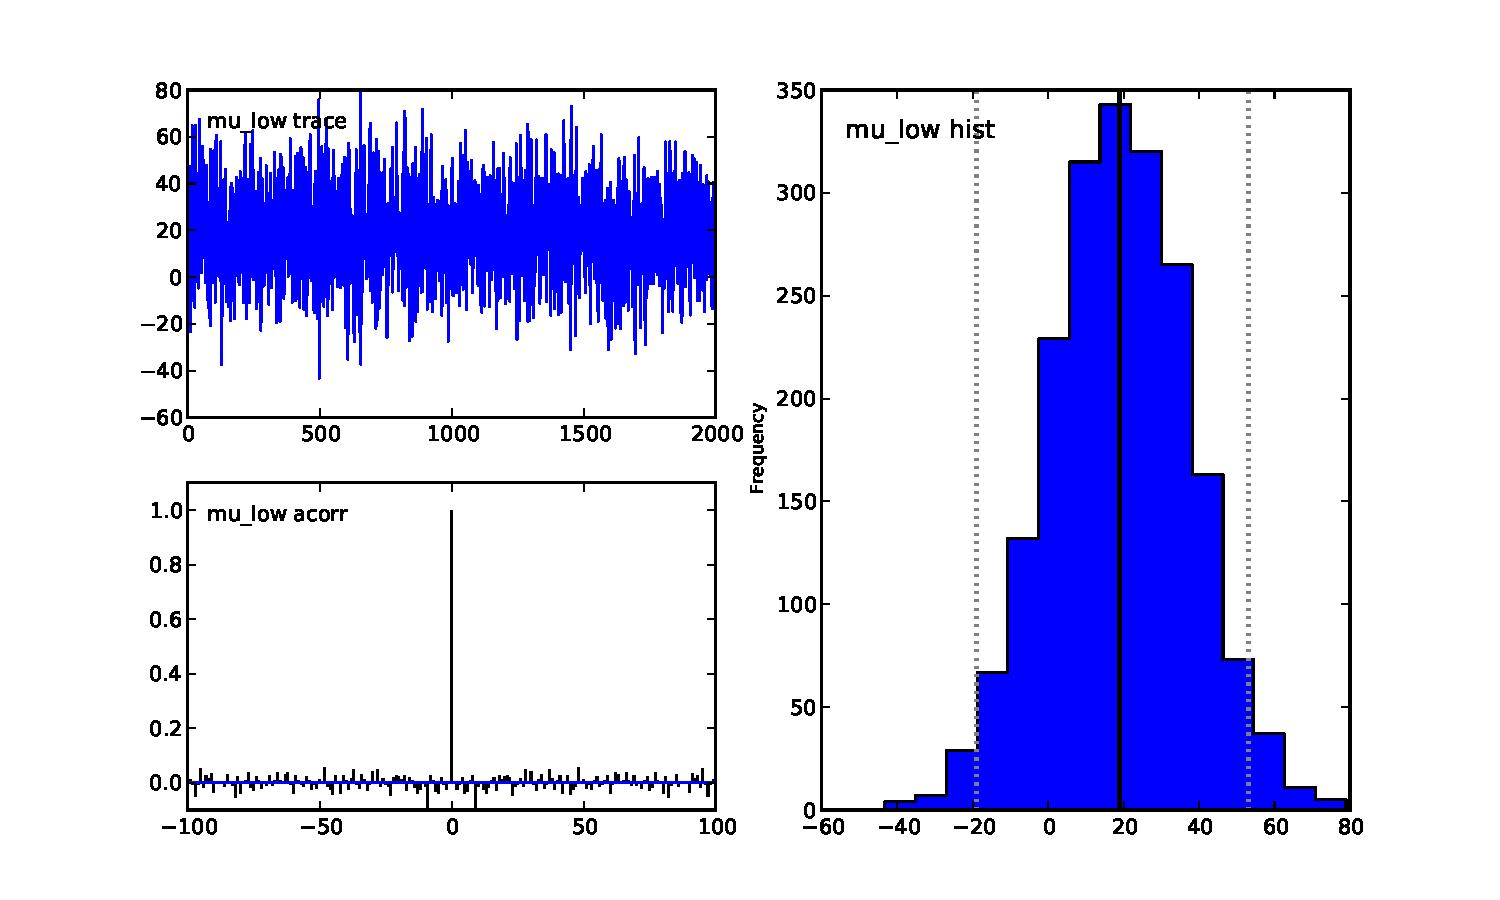
\includegraphics[height=2.0in]{./Figures/Prob7/Informed/mu_low} &
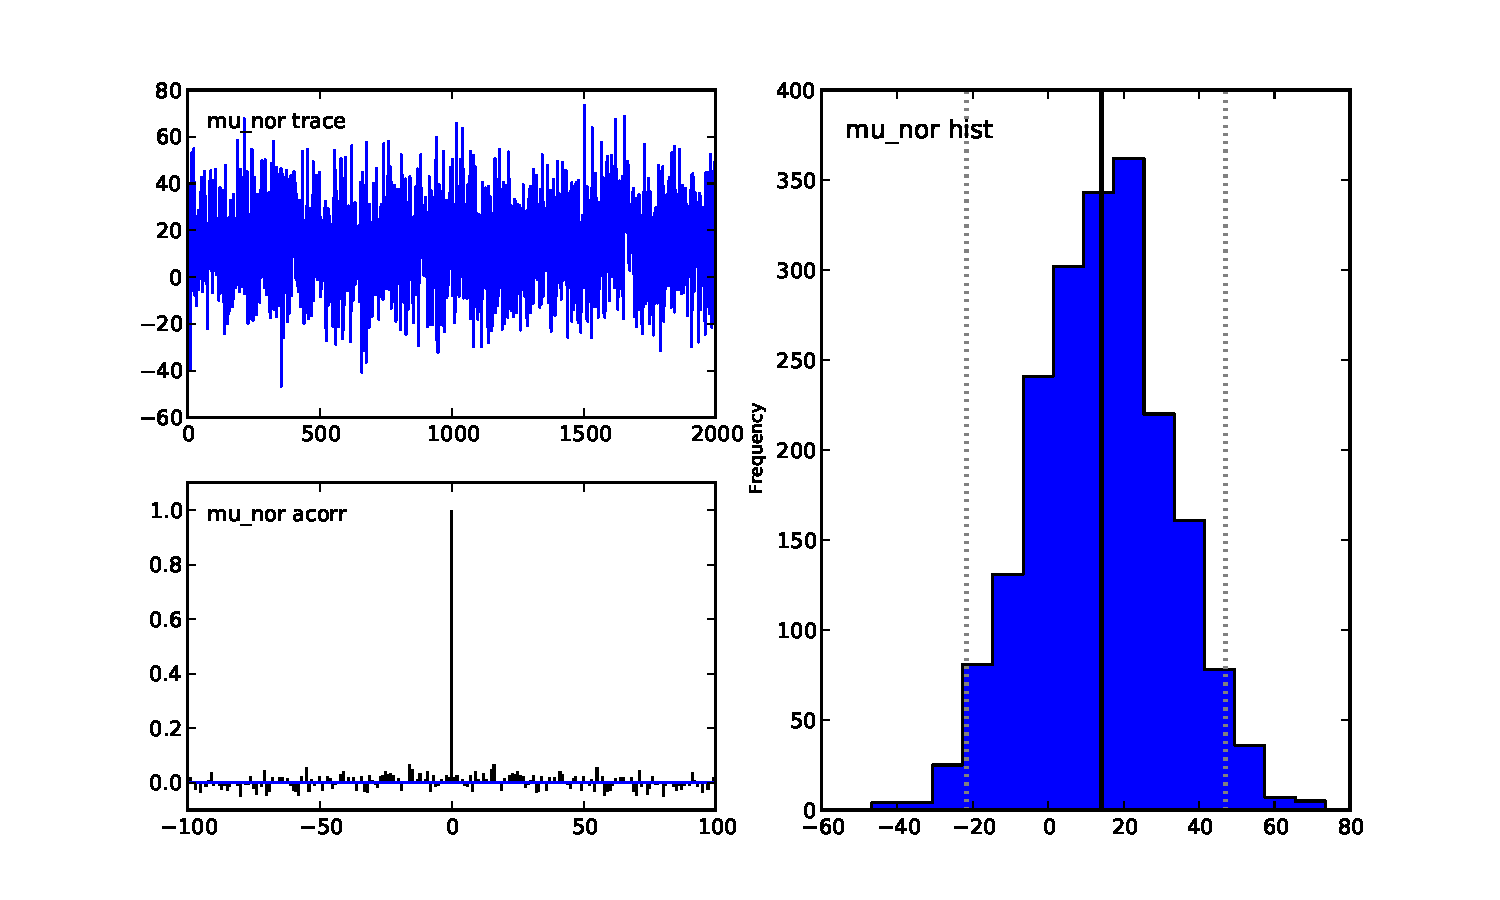
\includegraphics[height=2.0in]{./Figures/Prob7/Informed/mu_nor} \\
$\mu_1$ & $\mu_2$ \\
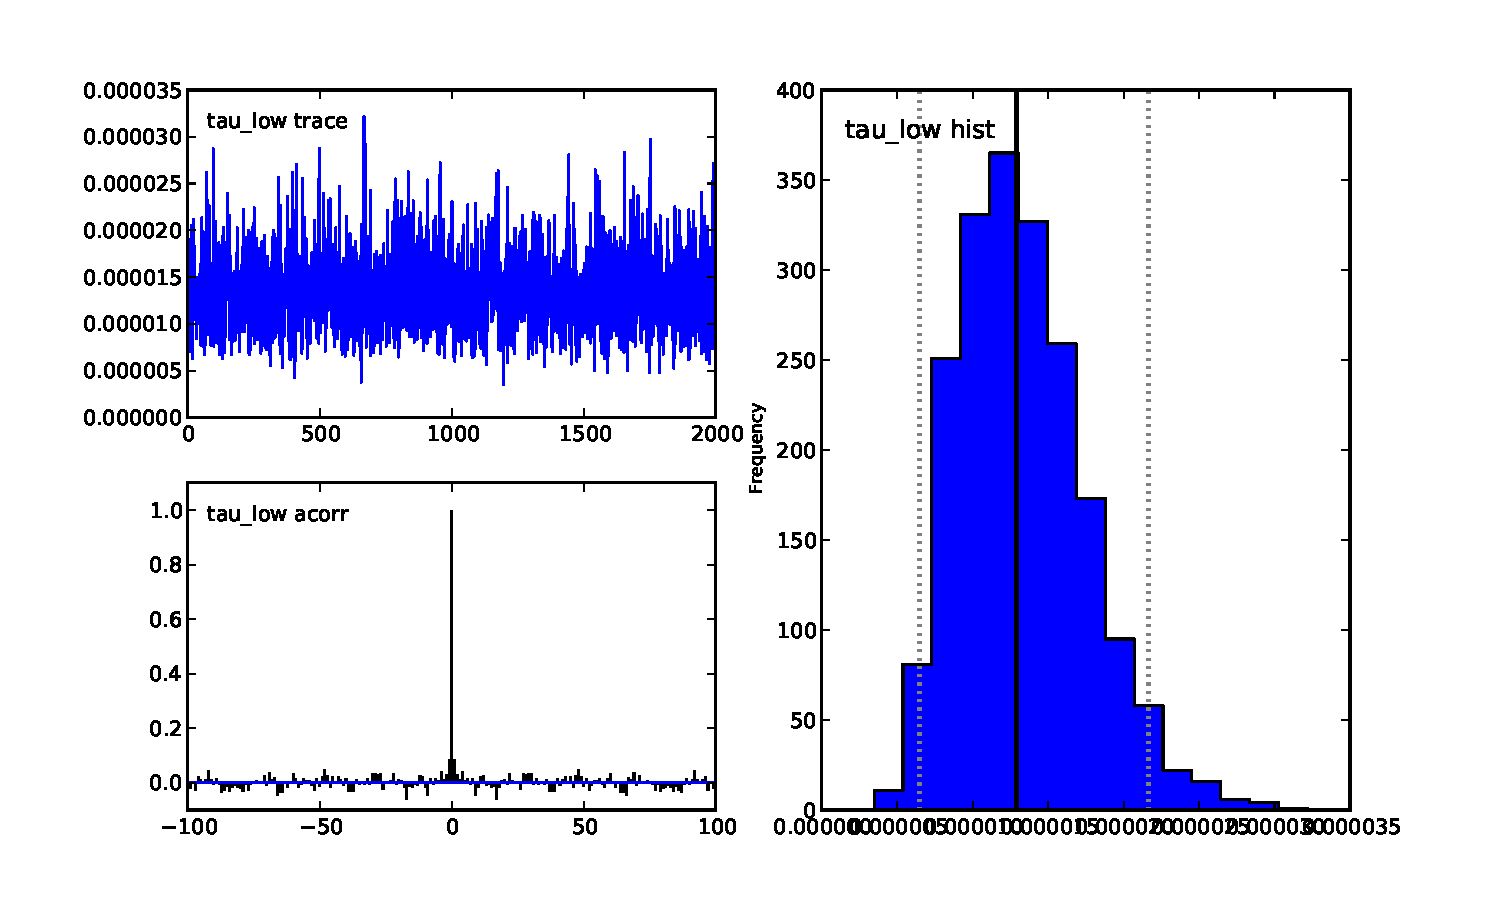
\includegraphics[height=2.0in]{./Figures/Prob7/Informed/tau_low} &
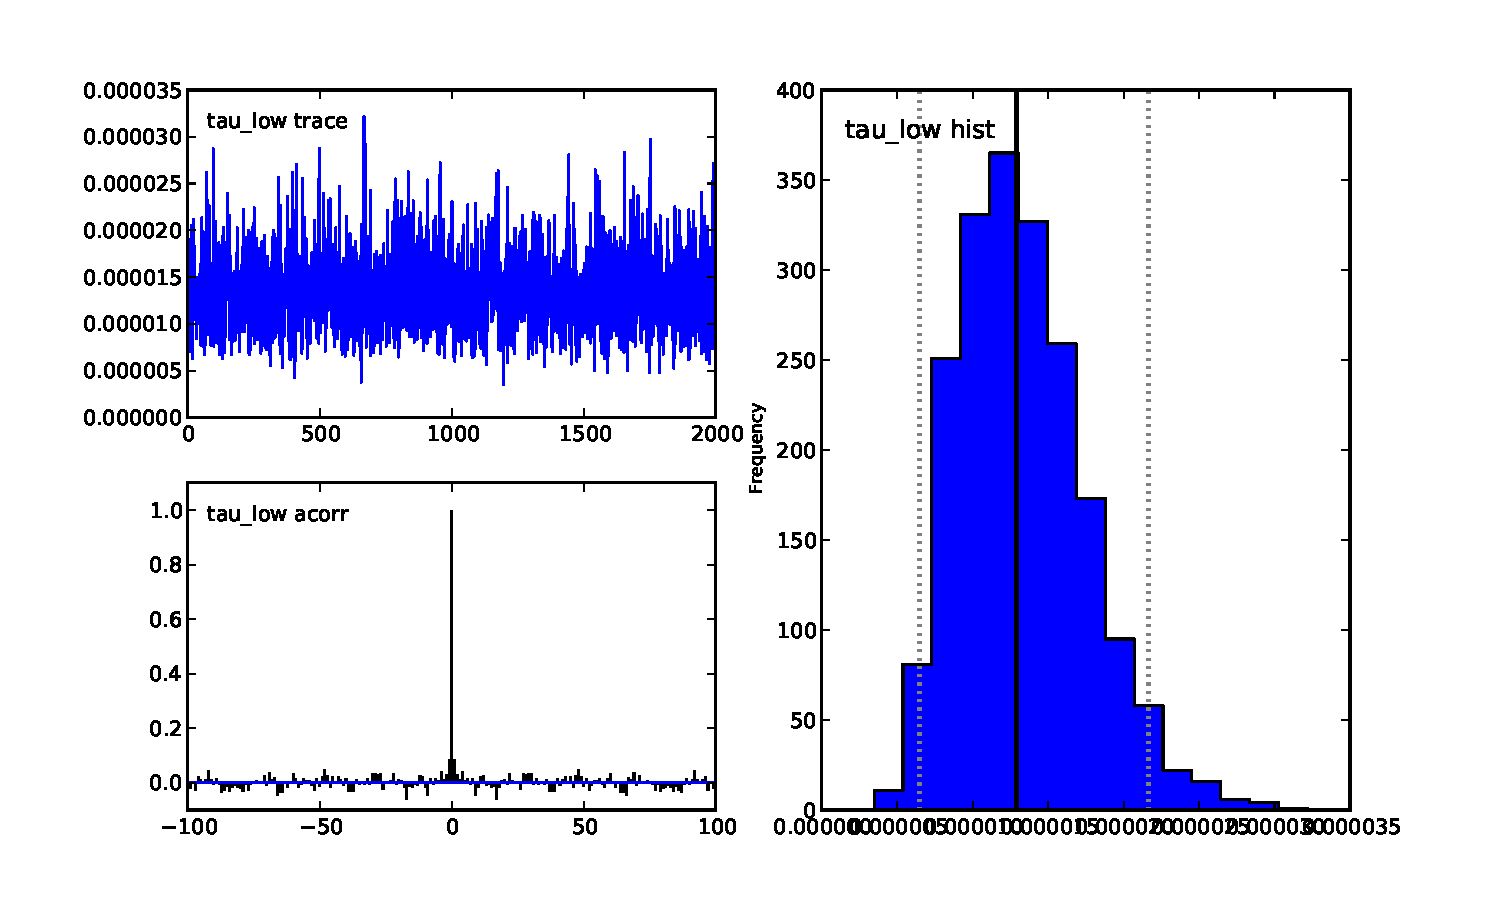
\includegraphics[height=2.0in]{./Figures/Prob7/Informed/tau_low} \\
$\tau_1$ & $\tau_2$ \\
\end{tabular}
\end{center}
\caption{Posteriors with Informed Priors}
\label{tab:p7_I}
\end{table}

\begin{table}[h!]
\begin{center}
\begin{tabular}{cc}
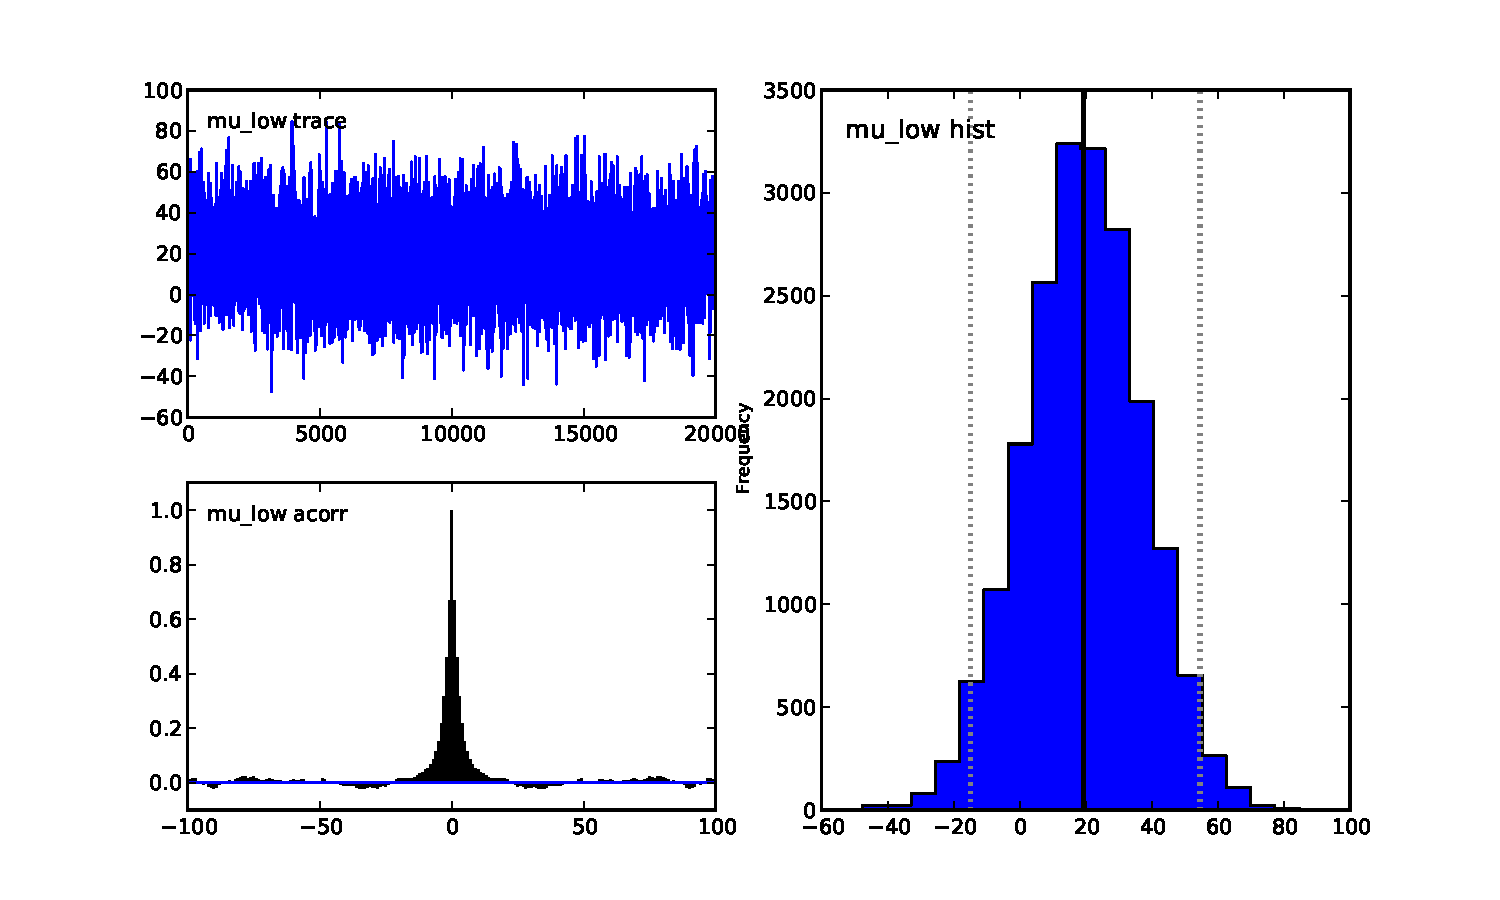
\includegraphics[height=2.0in]{./Figures/Prob7/Uninformed/mu_low} &
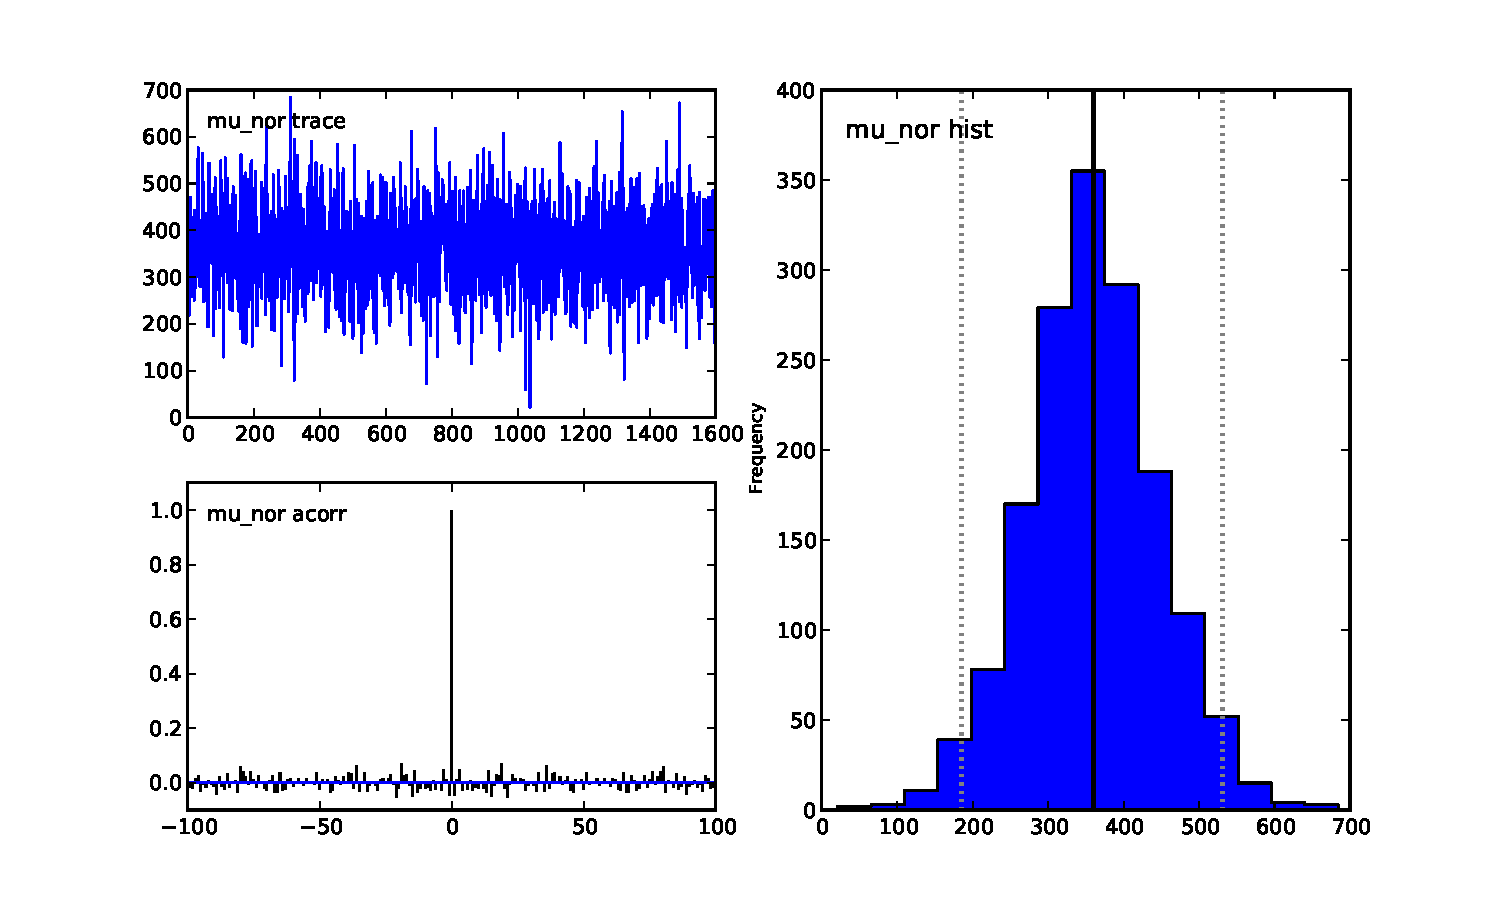
\includegraphics[height=2.0in]{./Figures/Prob7/Uninformed/mu_nor} \\
$\mu_1$ & $\mu_2$ \\
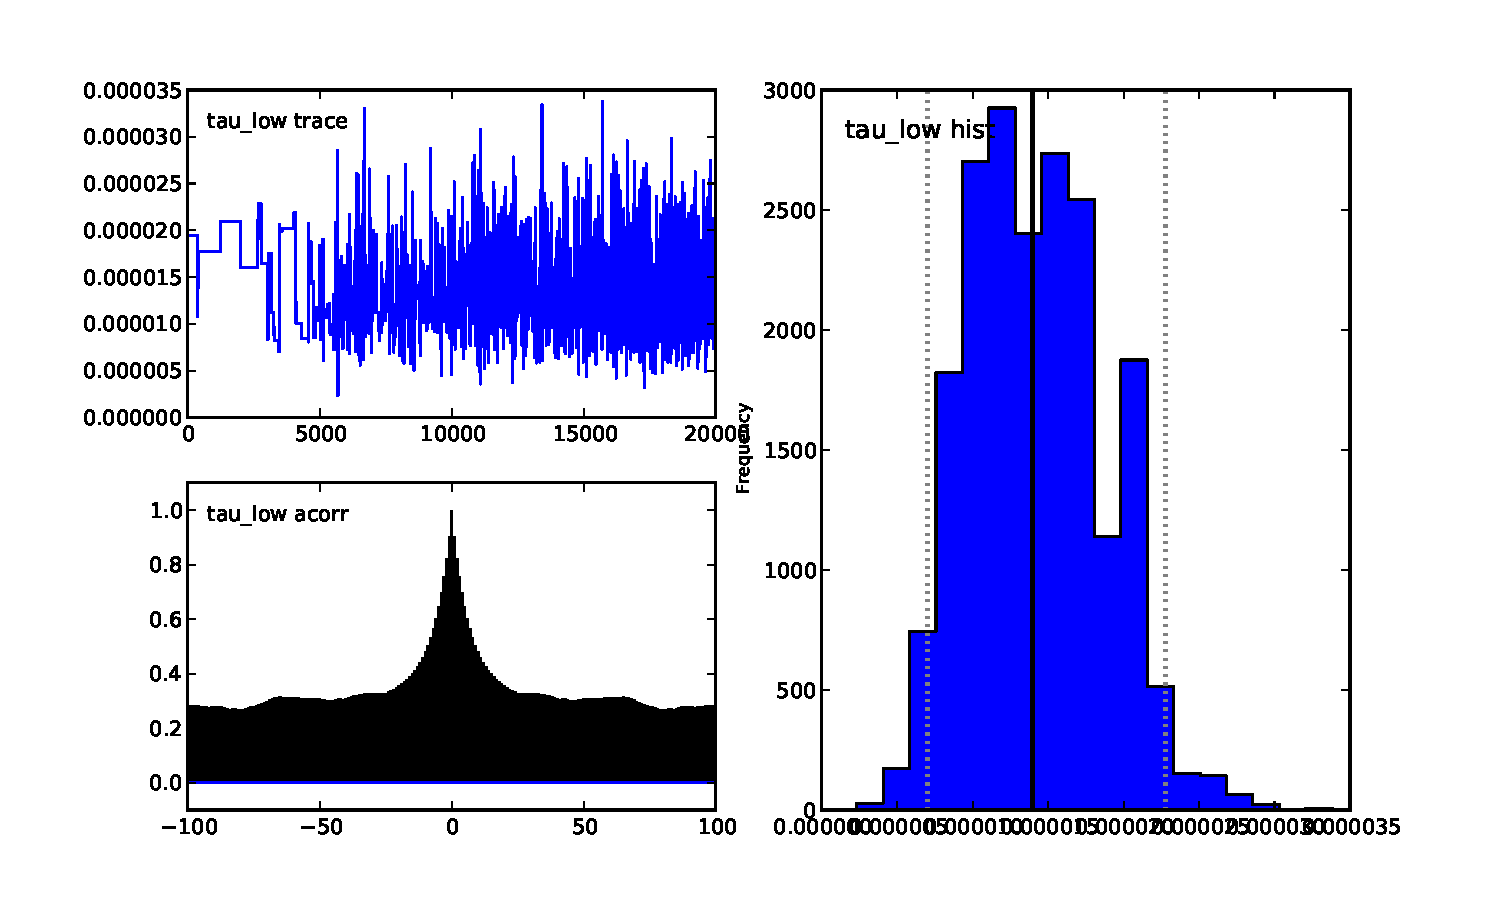
\includegraphics[height=2.0in]{./Figures/Prob7/Uninformed/tau_low} &
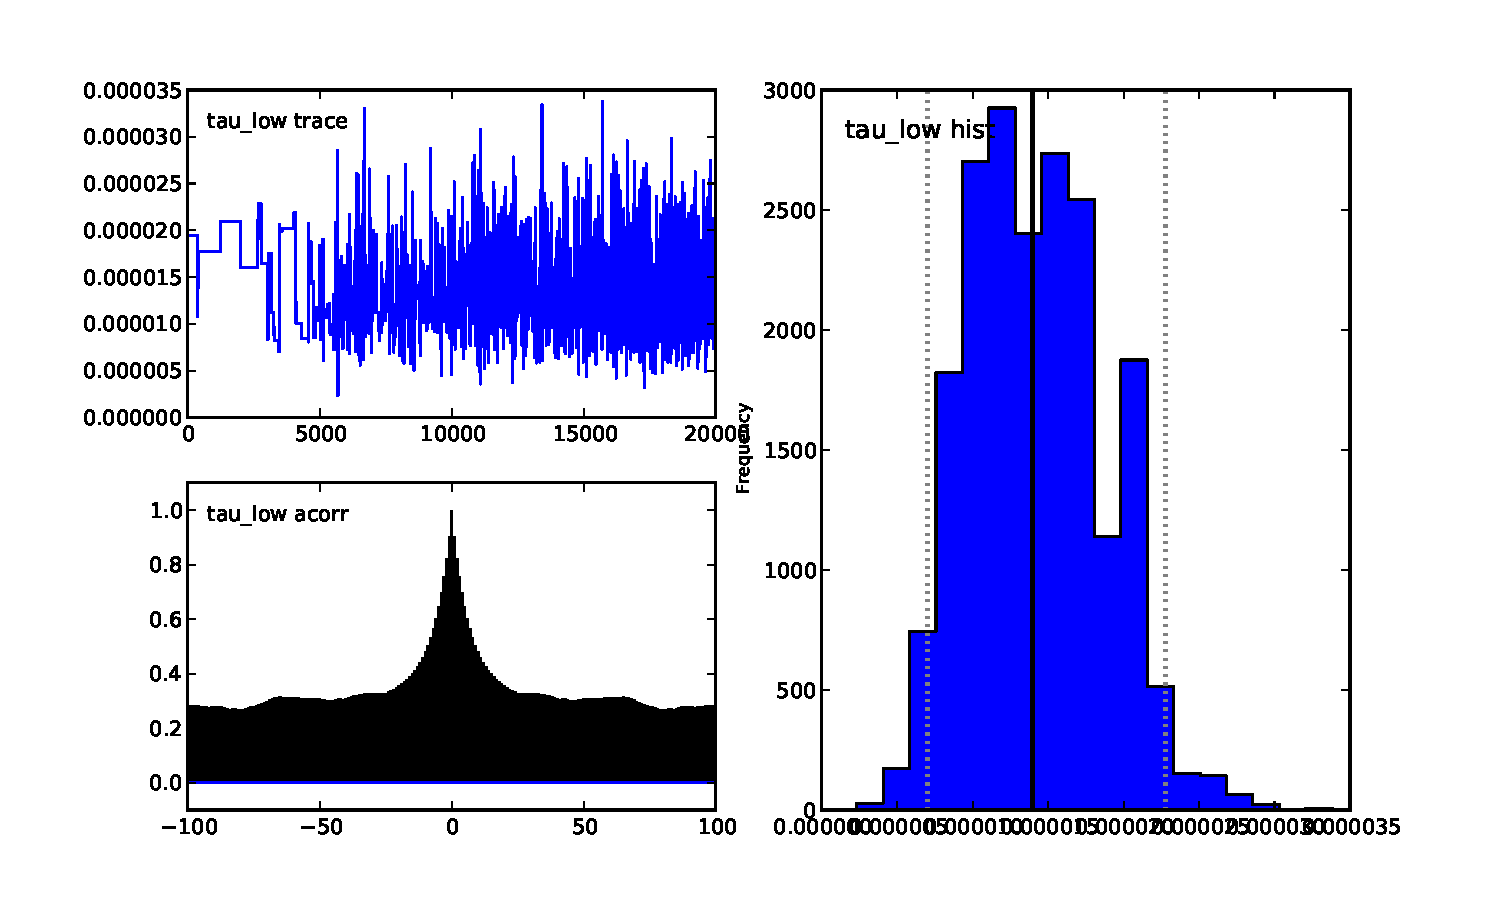
\includegraphics[height=2.0in]{./Figures/Prob7/Uninformed/tau_low} \\
$\tau_1$ & $\tau_2$ \\
\end{tabular}
\end{center}
\caption{Posteriors with Uninformed Priors}
\label{tab:p7_U}
\end{table}


\end{homeworkProblem}

\end{spacing}
\end{document}

%%%%%%%%%%%%%%%%%%%%%%%%%%%%%%%%%%%%%%%%%%%%%%%%%%%%%%%%%%%%%

%----------------------------------------------------------------------%
% The following is copyright and licensing information for
% redistribution of this LaTeX source code; it also includes a liability
% statement. If this source code is not being redistributed to others,
% it may be omitted. It has no effect on the function of the above code.
%----------------------------------------------------------------------%
% Copyright (c) 2007, 2008, 2009, 2010, 2011 by Theodore P. Pavlic
%
% Unless otherwise expressly stated, this work is licensed under the
% Creative Commons Attribution-Noncommercial 3.0 United States License. To
% view a copy of this license, visit
% http://creativecommons.org/licenses/by-nc/3.0/us/ or send a letter to
% Creative Commons, 171 Second Street, Suite 300, San Francisco,
% California, 94105, USA.
%
% THE SOFTWARE IS PROVIDED "AS IS", WITHOUT WARRANTY OF ANY KIND, EXPRESS
% OR IMPLIED, INCLUDING BUT NOT LIMITED TO THE WARRANTIES OF
% MERCHANTABILITY, FITNESS FOR A PARTICULAR PURPOSE AND NONINFRINGEMENT.
% IN NO EVENT SHALL THE AUTHORS OR COPYRIGHT HOLDERS BE LIABLE FOR ANY
% CLAIM, DAMAGES OR OTHER LIABILITY, WHETHER IN AN ACTION OF CONTRACT,
% TORT OR OTHERWISE, ARISING FROM, OUT OF OR IN CONNECTION WITH THE
% SOFTWARE OR THE USE OR OTHER DEALINGS IN THE SOFTWARE.
%----------------------------------------------------------------------%